\chapter{Classifier Guided Model}
\label{ch:classifier}


\section{Introduction}
\begin{tcolorbox}[colback=blue!10!white,colframe=blue!50!black,sharp corners]
Classifier guidance in diffusion models uses the gradients of an external image classifier to steer the generation process at each denoising step, forcing the model to produce images that strongly align with a specific target class.
\end{tcolorbox}

In \cite{jazbec_generative_2025} experiment, the ADM model was used without classifier guidance.
When reading the paper that introduced the \acs{ADM} model \parencite{dhariwal_diffusion_2021}, we see that adding classifier-guidance can significantly improve FID with a small cost on the recall. 

\section{Experiment}

The idea was to add the classifier to the ADM model that was missing in \cite{jazbec_generative_2025} experiment and run the same experiment as \autoref{ch:reproduce_adm}.

Additionally, \cite{jazbec_generative_2025} mentioned investigating the relation between Generative Uncertainty and classifier guidance as future work, so we hoped with this experiment to bring some answers.

\begin{tcolorbox}[colback=orange!10!white,colframe=orange!50!black,sharp corners]
Unfortunately, we realized after running the experiment that adding the classifier also changes the Bayesian framework and how the Laplace Approximation should be computed. We can therefore not really make conclusion on how the generative uncertainty method behaves with this classifier guided model.
Instead, we just observe observe how much adding this classifier improves the \acs{FPR} metrics compared to how filtering baseline were able to improve the \acs{FPR} metrics.
\end{tcolorbox}

\section{Observation}

\begin{figure}[!htbp]
    \centering
    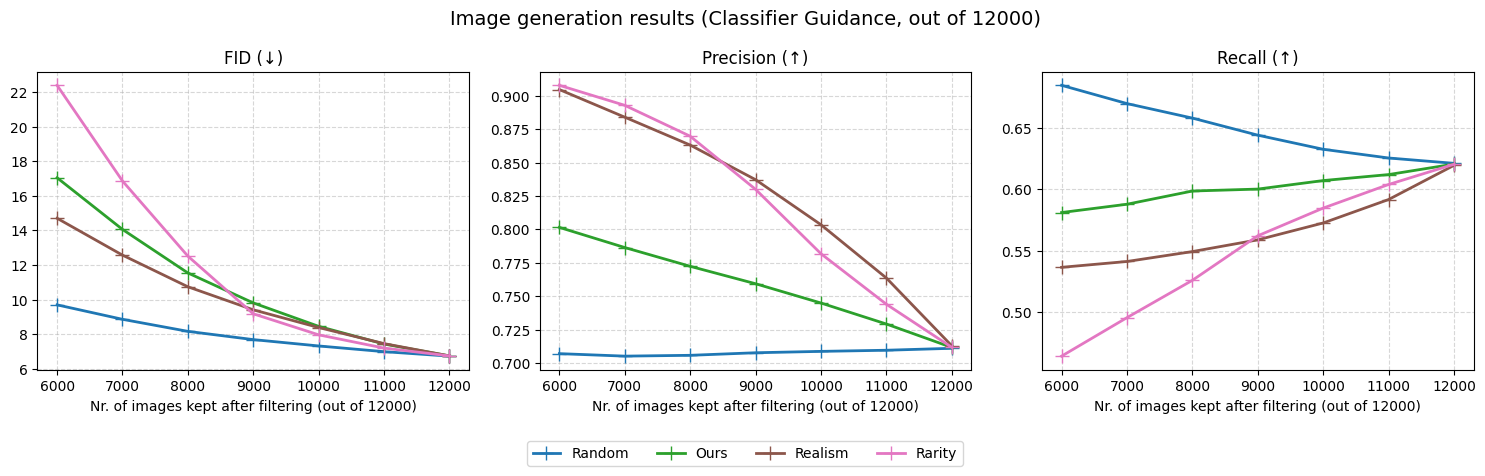
\includegraphics[width=0.99\linewidth]{figures/adm_experiment/classifier.png}
    \caption{Experiment results with classifier guidance. \warning to properly interpret those plots, we need to consider the sample size effect from \autoref{sub:problems_inception}, to account for that we look at the \textcolor{blue}{random baseline} and look at how much it departs from the horizontal line it should have ideally followed. Recall for instance looks better than it should at lower number of images kept}
    \label{fig:classifier}
\end{figure}


\autoref{fig:classifier} shows that without any filtering (keeping all 12000 images), we get as low as $FID \simeq 7$ which is far bellow what generative could provide being slightly bellow $FID \simeq 10$ when filtering out $2000$ images starting slightly bellow $FID \simeq 11$ without filtering \autoref{fig:classifier_free}.

We also observe that generative uncertainty (Ours) struggles to really improve the \acs{FPR} metrics (especially on the FID) 
% (even when considering the sample size problem in \autoref{sub:problems_inception} that naturally)
which can be partially explained when considering the note above on how we should have adapted the Laplace approximation implementation to consider the classifier effects. But we observe the same problem with Realism and Rarity which should not be affected by the Bayesian framework but only the validation and generated datasets. This indicates that adding the classifier might actually render filtering methods ineffective or simply make them redundant. On FID for instance the \texttt{random} baseline outperforms everything.

Although we see a significant rise in precision, it occurs at an high cost of recall.

\section{Conclusion}
Fortunately filtering metrics will remain useful because even if the model generates far less artifacts, we still need to detect them. But from the perspective of trying to improve the quality of a generated dataset it seems like adding the classifier is the way to go, with the added advantage of not having to generate more images to filter out the worse ones.

% It seems like the uncertainty tail as we observed in the toy experiment has disappeared with classifier-guided generations. To verify this, we run the same uncertainty plot on this experiment and get \autoref{fig:uncertainty_dist_adm}. We don't observe a clean and isolated \textit{tail of uncertainty}. But we still observe a skew in the distribution, the samples have been pushed left (less uncertain).

% This lack of clean tail of uncertainty might be caused by overly aggressive approximations made to render the generative uncertainty computation feasible on large models in \parencite{jazbec_generative_2025}, we will later explore the impact of those approximations on the toy experiment first and try to improve it's accuracy with reasonable computational cost.

% \begin{figure}[!htbp]
%     \centering
%     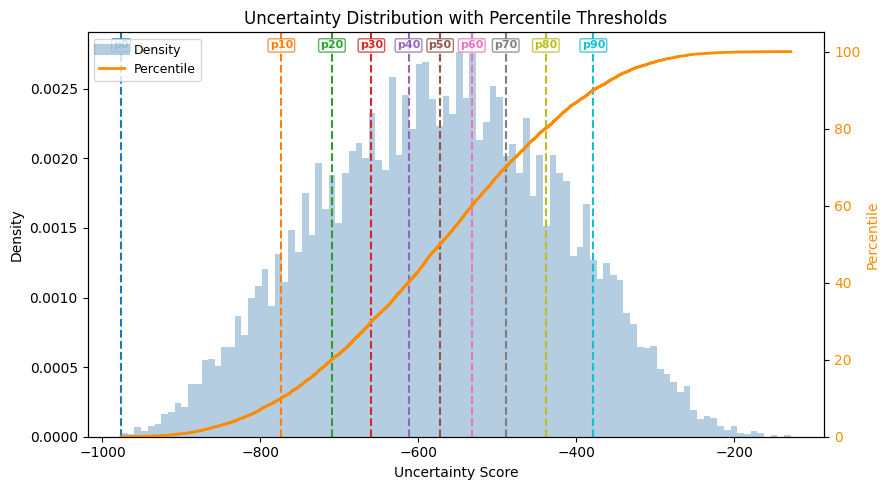
\includegraphics[width=0.49\linewidth]{figures/adm_experiment/uncertainty_classifier_free.png}
%     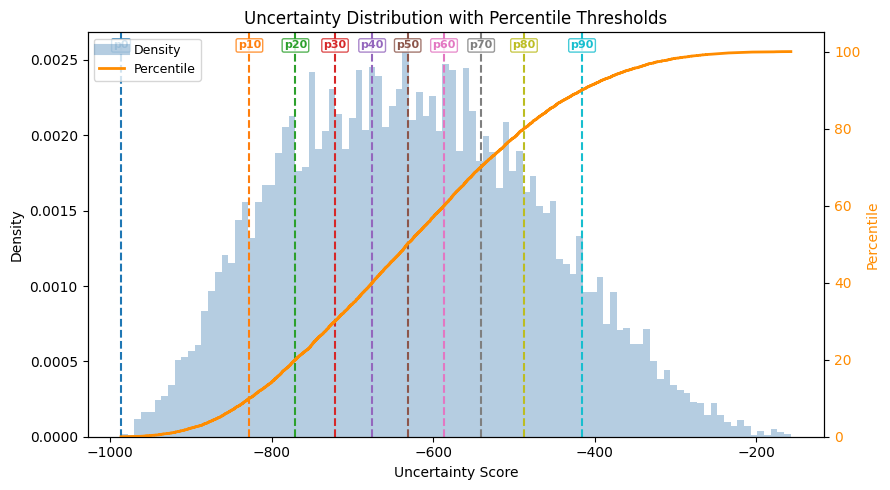
\includegraphics[width=0.49\linewidth]{figures/adm_experiment/uncertainty_classifier.png}
%     \caption{Uncertainty distribution for the ADM model generations. On the left: classifier free guidance, on the right: classifier guidance}
%     \label{fig:uncertainty_dist_adm}
% \end{figure}

% \section{Conclusion}

% ... Relying on a classifier to improve the score is nice and performs much better than any filtering metrics but it's not a replacement for generative uncertainty